\section{Additional Figures}

\begin{figure*}
    \centering
    \begin{subfigure}{\columnwidth}
        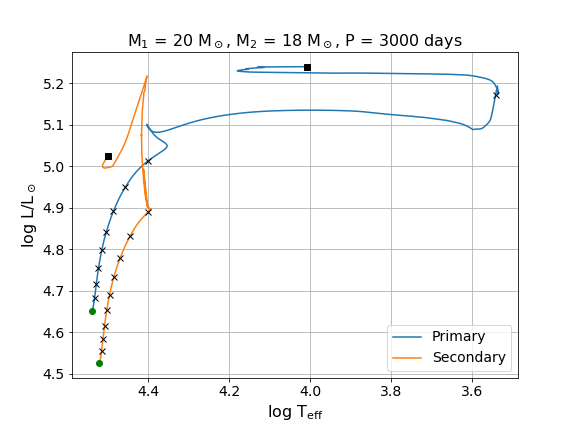
\includegraphics[width=\columnwidth]{figures/results1/fig_HR_M20_P3000.png}
        \label{subfig:20Msol_P3000_HR}
    \end{subfigure}
    \begin{subfigure}{\columnwidth}
        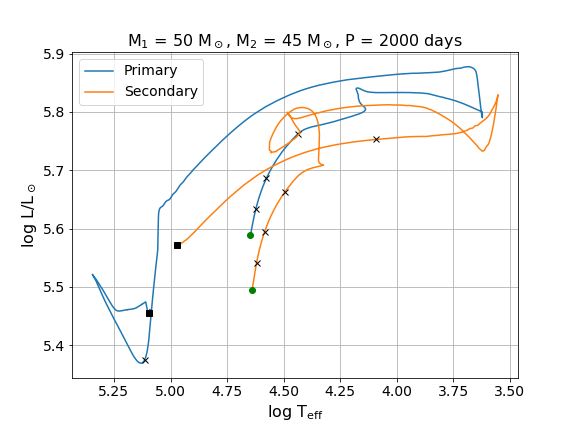
\includegraphics[width=\columnwidth]{figures/results1/fig_HR_M50_P2000.png}
        \label{subfig:50Msol_P2000_HR}
    \end{subfigure}
    
    \begin{subfigure}{\columnwidth}
        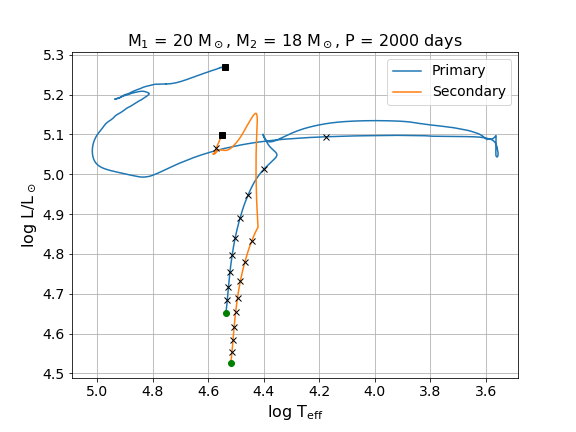
\includegraphics[width=\columnwidth]{figures/results1/fig_HR_M20_P2000.png}
        \label{subfig:20Msol_P2000_HR}
    \end{subfigure}
    \begin{subfigure}{\columnwidth}
        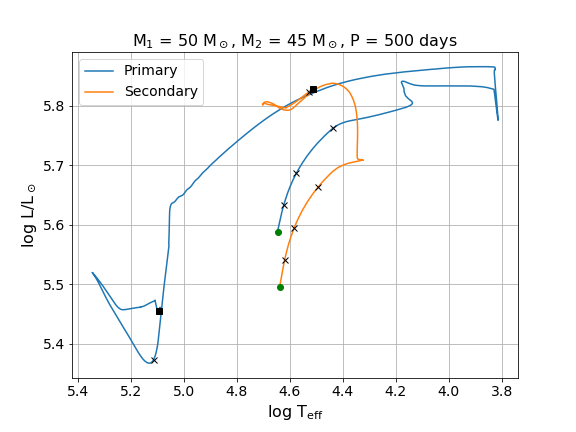
\includegraphics[width=\columnwidth]{figures/results1/fig_HR_M50_P500.png}
        \label{subfig:50Msol_P500_HR}
    \end{subfigure}
    
    \begin{subfigure}{\columnwidth}
        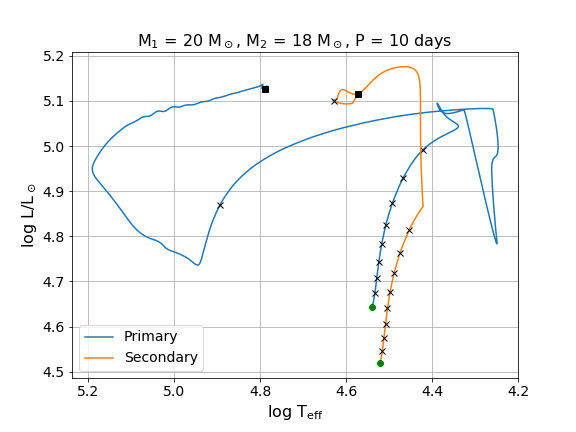
\includegraphics[width=\columnwidth]{figures/results1/fig_HR_M20_P10.png}
        \label{subfig:20Msol_P10_HR}
    \end{subfigure}
    \begin{subfigure}{\columnwidth}
        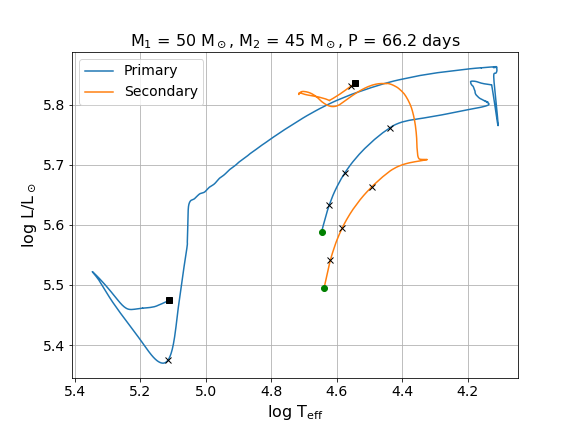
\includegraphics[width=\columnwidth]{figures/results1/fig_HR_M50_P66.png}
        \label{subfig:50Msol_P66_HR}
    \end{subfigure}
    
\caption{HR diagrams comparing the evolution of M$_1$ = 20 M$_\sun$ (left) and M$_1$ = 50 M$_\sun$ (right) binary systems at different initial periods. The shorter the period, the sooner in their evolution RLOF occurs. Note that as massive stars have higher luminosities, the secondary tracks move upwards as mass is accreted. The HR diagrams are as figure \ref{fig:SinglevsBinary}. For the M$_1$ = 20 M$_\sun$ system, mass transfer was case C (RLOF during helium-burning) for P > 2000 days, and case B for 10 < P < 2000 days. P = 2000 days provided an edge case where RLOF coincided with the ignition of helium. For the M$_1$ = 50 M$_\sun$ system, mass transfer was case B for P > 10 days, and case A for P = 10 days (not pictured). In this latter simulation, both stars filled their Roche lobes simultaneously, forming a contact binary and rendering the HR diagram invalid beyond that point. Note that for P = 2000, the secondary's accretion is limited enough that it begins its WR evolution even after rejuvenation of core hydrogen extends its main sequence lifespan.}
\label{fig:Period_HR}
\end{figure*}

\begin{figure*}
    \centering
    \begin{subfigure}{\columnwidth}
        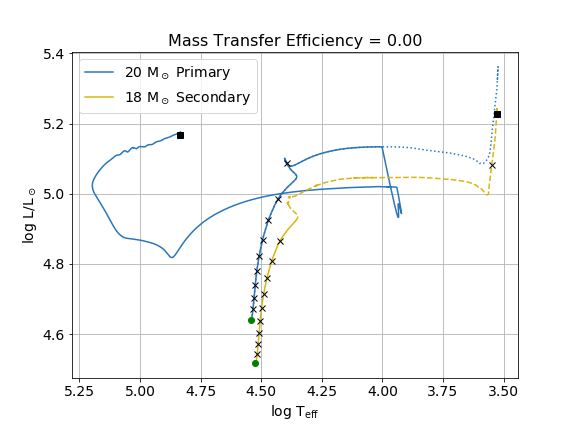
\includegraphics[width=\columnwidth]{figures/results2/fig_HR_MassTransfer_0.png}
        \label{subfig:MTE0_HR}
    \end{subfigure}
    \begin{subfigure}{\columnwidth}
        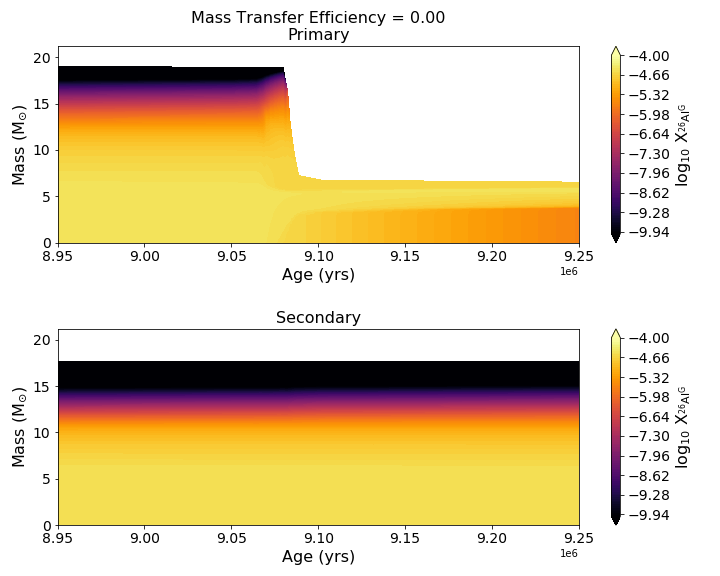
\includegraphics[width=\columnwidth]{figures/results2/fig_Al26_MassTransfer_0.png}
        \label{subfig:MTE0_Al26}
    \end{subfigure}
    
    \begin{subfigure}{\columnwidth}
        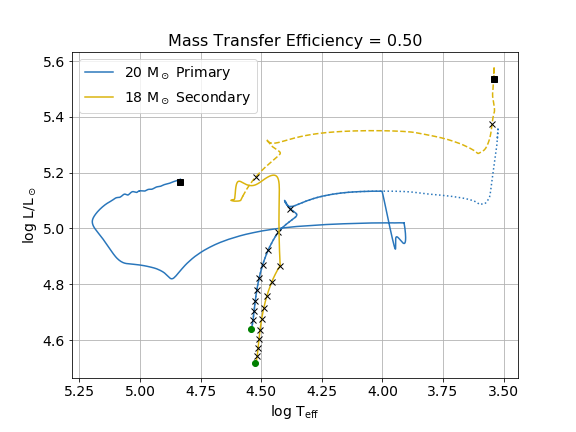
\includegraphics[width=\columnwidth]{figures/results2/fig_HR_MassTransfer_50.png}
        \label{subfig:MTE50_HR}
    \end{subfigure}
    \begin{subfigure}{\columnwidth}
        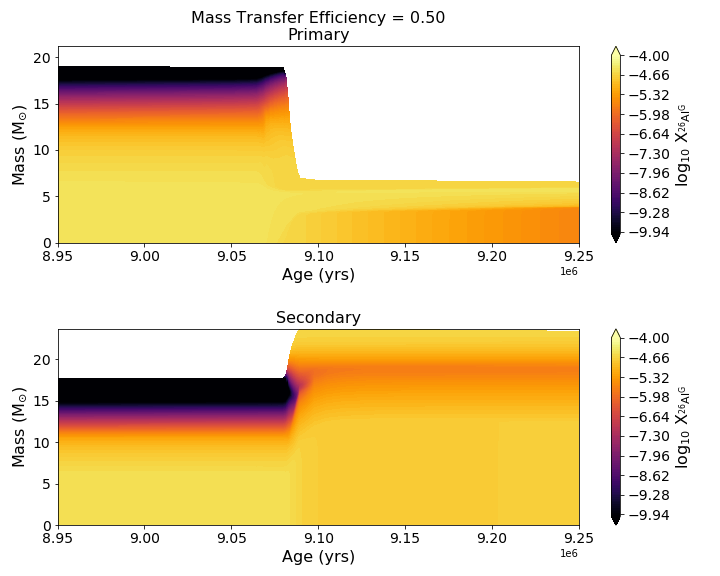
\includegraphics[width=\columnwidth]{figures/results2/fig_Al26_MassTransfer_50.png}
        \label{subfig:MTE50_Al26}
    \end{subfigure}
    
    \begin{subfigure}{\columnwidth}
        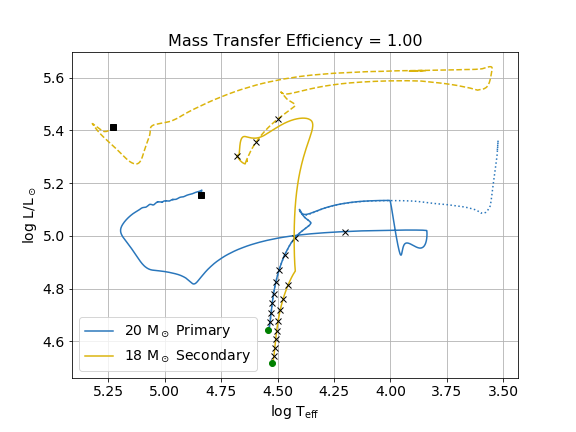
\includegraphics[width=\columnwidth]{figures/results2/fig_HR_MassTransfer_100.png}
        \label{subfig:MTE100_HR}
    \end{subfigure}
    \begin{subfigure}{\columnwidth}
        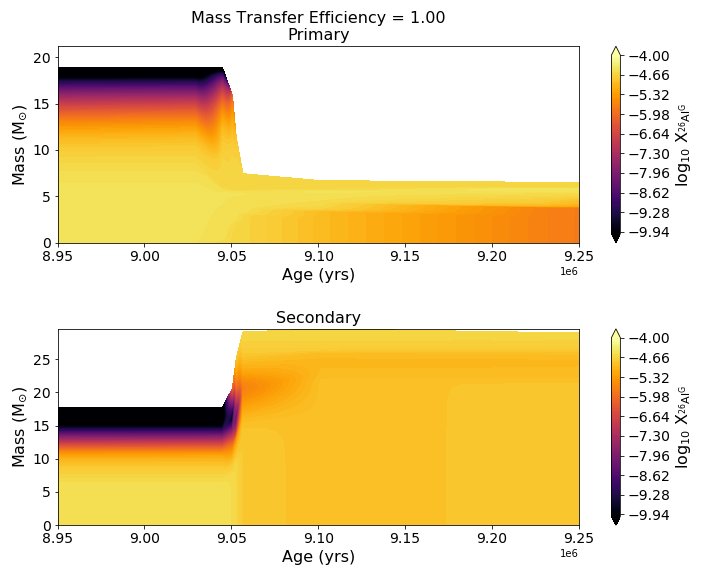
\includegraphics[width=\columnwidth]{figures/results2/fig_Al26_MassTransfer_100.png}
        \label{subfig:MTE100_Al26}
    \end{subfigure}
\caption{HR diagrams (left) and $^{26}$Al composition diagrams (right) comparing the evolution of binary stars undergoing non-conservative mass transfer (top), partially conservative mass transfer (middle), and fully conservative mass transfer (bottom).
For the HR diagrams: the dotted blue line depicts the evolution track of a single star counterpart to the primary, and the dashed yellow line shows the continued single-star evolution of the secondary star after mass transfer.
The composition diagrams are as figures \ref{fig:20Msol_Composition} \& \ref{fig:50Msol_Composition}, but focused only on the RLOF stage of evolution.
Each simulation has initial primary mass 20 M$_{\sun}$, mass ratio q = 0.9, and initial orbital period P = 100 days.}
\label{fig:MTE_HR}
\end{figure*}